\documentclass[12pt]{article}
\usepackage[top=0.9in, bottom=0.9in, left=0.9in, right=1.1in]{geometry}

\usepackage{graphicx,color,enumitem}
\usepackage{amsmath,amsthm,amsbsy}
\usepackage{palatino}

\usepackage{tikz}

%% Setup aproblem environment, 
%% aproblem items
%% subproblems environment
%% subproblem items
\makeatletter
\newcounter{probcount}
\newcounter{subprobcount}
\newlength\probsep
\newlength\pshrinking
\newif\iffirstprob

\newenvironment{aproblems}%
  {\ifhmode\unskip\par\fi\setcounter{probcount}{0}\probsep\parskip
  \sbox\@tempboxa{\textbf{9.}}\pshrinking\wd\@tempboxa\advance\pshrinking\labelsep
  \let\hproblem\aproblem
  \advance\linewidth -\pshrinking
  \advance\@totalleftmargin\pshrinking
  \advance\leftskip\pshrinking}%
  {\ifhmode\unskip \par\fi\advance\leftskip-\pshrinking}%

\newcommand{\aproblem}{%
  \setcounter{subprobcount}{0}%
  \stepcounter{probcount}%
  \def\@currentlabel{\arabic{probcount}}%
  \ifhmode
    \unskip \par
  \fi
%  \addpenalty{-4000}%
  \iffirstprob\else\addvspace\probsep\fi
  \firstprobfalse
  \hskip -\labelwidth\hskip -\labelsep 
  \hbox to\labelwidth{\hss\textbf{\arabic{probcount}.}}\hskip\labelsep
}%

\newcommand{\subprob}{\item\def\@currentlabel{\arabic{probcount}\alph{\thelistlabel}}}
\newcommand{\skipproblem}{\stepcounter{probcount}}


%% The following commands put defined left and right headers on the top, and a page number
%% on the bottom of all pages beyond page 1
\usepackage{fancyhdr}
\pagestyle{fancy}
\fancyfoot[C]{\ifnum \value{page} > 1\relax\thepage\fi}
\fancyhead[L]{\ifx\@doclabel\@empty\else\@doclabel\fi}
\fancyhead[R]{\ifx\@docdate\@empty\else\@docdate\fi}
\headheight 15pt
\def\doclabel#1{\gdef\@doclabel{#1}}
\def\docdate#1{\gdef\@docdate{#1}}
\makeatother

%% General formatting parameters
\parindent 0pt
\parskip 6pt plus 1pt


\doclabel{Math F251: Section 4.9 Worksheet}
\docdate{Friday 9 November 2018}


\begin{document}
\renewcommand{\d}{\displaystyle}

\begin{aproblems}

% 4.9 # 11, 17, 21
\aproblem  Find the most general antiderivative of the function.  (\emph{Check your answer by differentiation.})

\renewcommand{\labelenumi}{\textbf{(\alph{enumi})}}
\begin{enumerate}
\item $f(x) = 3 \sqrt{x} - 2\sqrt[3]{x}$

\vfill
\item $h(\theta) = 2 \sin \theta - \sec^2 \theta$

\vfill
\item % change to include \ln x
    $$f(x) = \frac{2x^4+4x^3-x^2}{x^3}, \qquad x>0 \hspace{5.0in}$$
\end{enumerate}
\vfill

\newpage
\thispagestyle{plain}

% 4.9 # 33, 40
\aproblem  Find $f$.
\renewcommand{\labelenumi}{\textbf{(\alph{enumi})}}
\begin{enumerate}
\item $f'(t) = 4/(1+t^2)$, \, $f(1)=0$

\vfill
\item $f''(x)=8x^3+5$, \, $f(1)=0$, \, $f'(1)=8$

\end{enumerate}
\vfill

% 4.9 # 55
\aproblem  The graph of $f'$ is shown in the figure.  Sketch the graph of $f$ if $f$ is continuous and $f(0)=-1$.

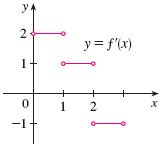
\includegraphics[width=0.3\textwidth]{stepfcn}
\vfill

\end{aproblems}

\end{document}
